\section*{Model following control}
\addcontentsline{toc}{section}{Model following control}

\subsection*{Level 1}
\addcontentsline{toc}{subsection}{Level 1}

Here, we will design a model following controller by inverting the process model in the time domain.

The control structure and the model following block are depicted in Figure \ref{contStruct}.

\begin{figure}[t!p]
\begin{center}
  \begin{subfigure}[b]{\columnwidth}
  \includegraphics[trim=125 40 150 40,clip=true,height=\linewidth,angle=270]{fig/modelFollowing.eps}
 \caption{Model following for the DC-motor}
  \end{subfigure}
    \begin{subfigure}[b]{\columnwidth}
  \includegraphics[trim=125 0 150 25,clip=true,height=\linewidth,angle=270]{fig/modelMotorServo1.eps}
   \caption{Control structure for the DC-motor}
  \end{subfigure}
  \caption{Model following and control structure for a DC-motor}
 \label{contStruct}
\end{center}
\end{figure}

Since the DC-motor model we used is a second order system, the reference position must be two times differentiable. 

The trajectory planner is design using the fastest possible positionning:
\begin{equation}a_{max} = \frac{\pm M_{max}}{J}\end{equation}
\begin{equation}v_{max} = \pm \frac{U_{max} - \frac{R}{k_\varphi} F_c}{\frac{R d}{k_\varphi} + k_\varphi}\end{equation}

With:

$M_{max}$ : maximum torque of the motor

$v_{max}$ : maximum reachable velocity of the DC-motor, computed with the DC motor model equations.

The reference signal is computed using the following equations:

  Let $t_1 = \frac{v_{max}}{a_{max}}, t_2 = \frac{Rs}{v_{max}}  \text{ and } t_1' = \sqrt{\frac{Rs}{a_{max}}}$\\
  \begin{equation}
  a(t) = \left\{ \begin{array}{lcl} a_{max} & , & t < t_1 \\
				      0 & , & t_1 < t < t_2 \\ 
				  -a_{max} &,& t_2 < t < t_1 + t_2 \\
				  0 & , & t>t_1 + t_2
		  \end{array} \right.\text{ , if } t_1 < t_2
  \end{equation}
  \begin{equation}
  a(t) = \left\{ \begin{array}{lcl} a_{max} & , & t < t_1' \\
				  -a_{max} &,& t_1' < t < 2t_1'\\
				  0 & , & t>2t_1'
		  \end{array} \right.\text{ , if } t_1 > t_2
  \end{equation}


The reference signal is then created as depicted in Figure \ref{trajplan}.

\begin{figure}[t!p]
  \begin{center}

  \begin{subfigure}[b]{\columnwidth}
  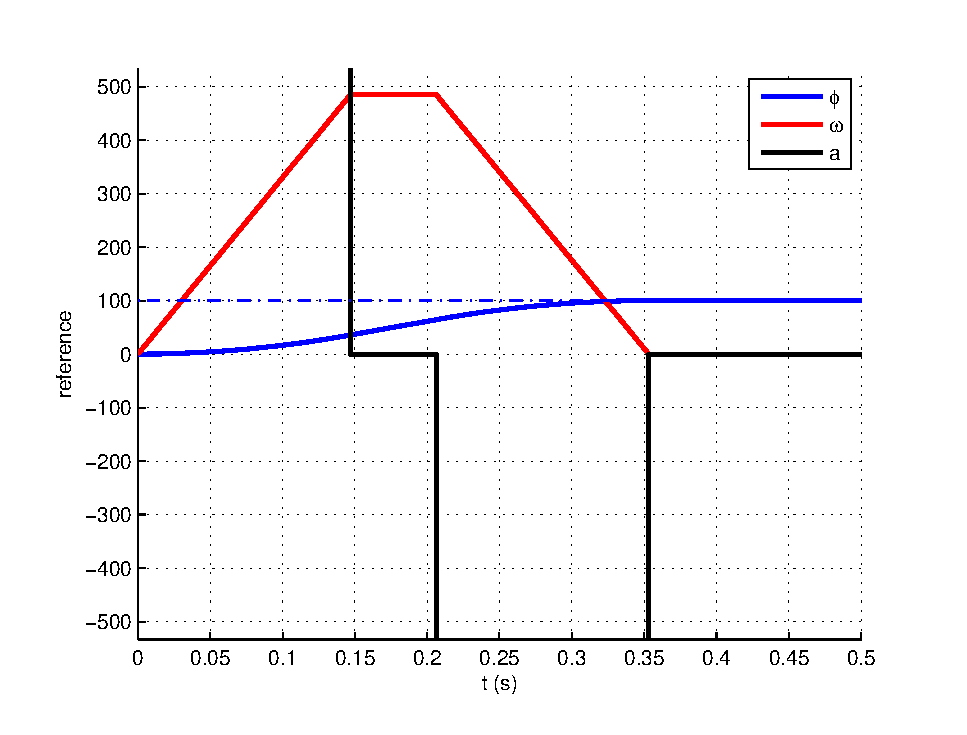
\includegraphics[width = \columnwidth]{fig/trajPlanref100.eps}
  \caption{Reference signal for $Rs = 100$ [rad]}
  \end{subfigure}
  \vspace{\fill}
  \begin{subfigure}[b]{\columnwidth}
  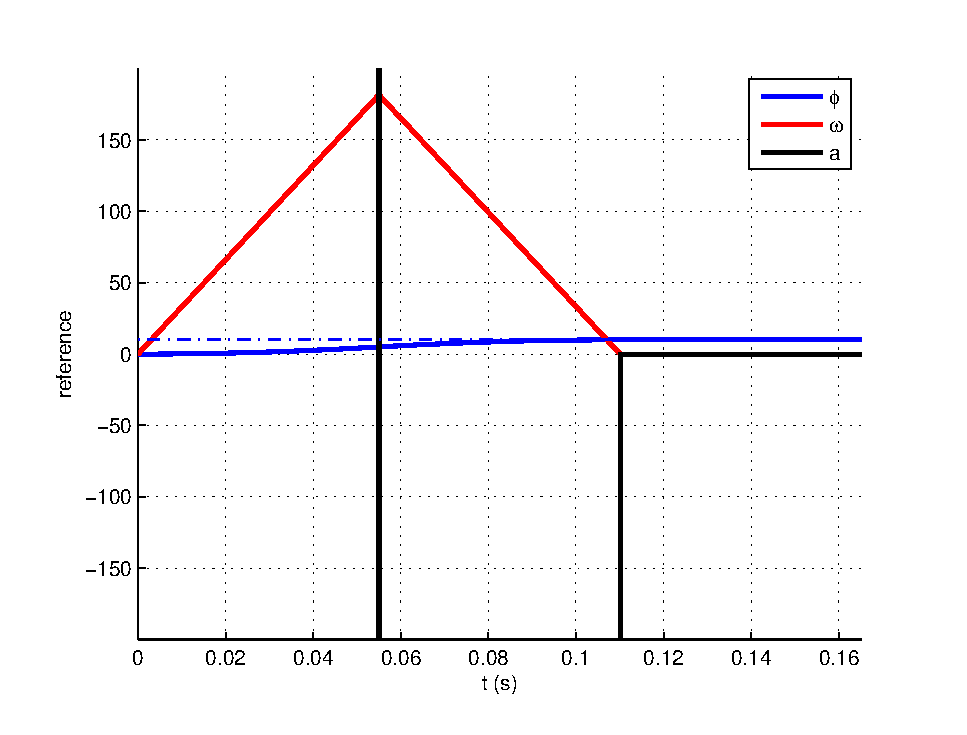
\includegraphics[width = \columnwidth]{fig/trajPlanref10.eps}
  \caption{Reference signal for $Rs = 10$ [rad]}
  \end{subfigure}
\caption{Reference signal}
\label{trajplan}
\end{center}
\end{figure}


Once the reference signal is designed, we simulate the system (simulation and real-case). Figure \ref{resultModelfollowing} shows the results.
 
The Servo control model leads to an excellent control law of the motor for the two set points. Since the trajectory computed by the trajectory planner is completly reachable by the real-motor (no saturation), the planned trajectory and the real one are almost completly merged.

\textbf{Remark:} In order to be sure of our control design, we reduced the value of $a_{max}$ and $v_{max}$ to $75\%$ of the value computed theoretically. Indeed, using the maximum value of those value drive the motor to a dangerous area.

\begin{figure}[ht]
  \centering
  \begin{subfigure}[b]{\linewidth}
   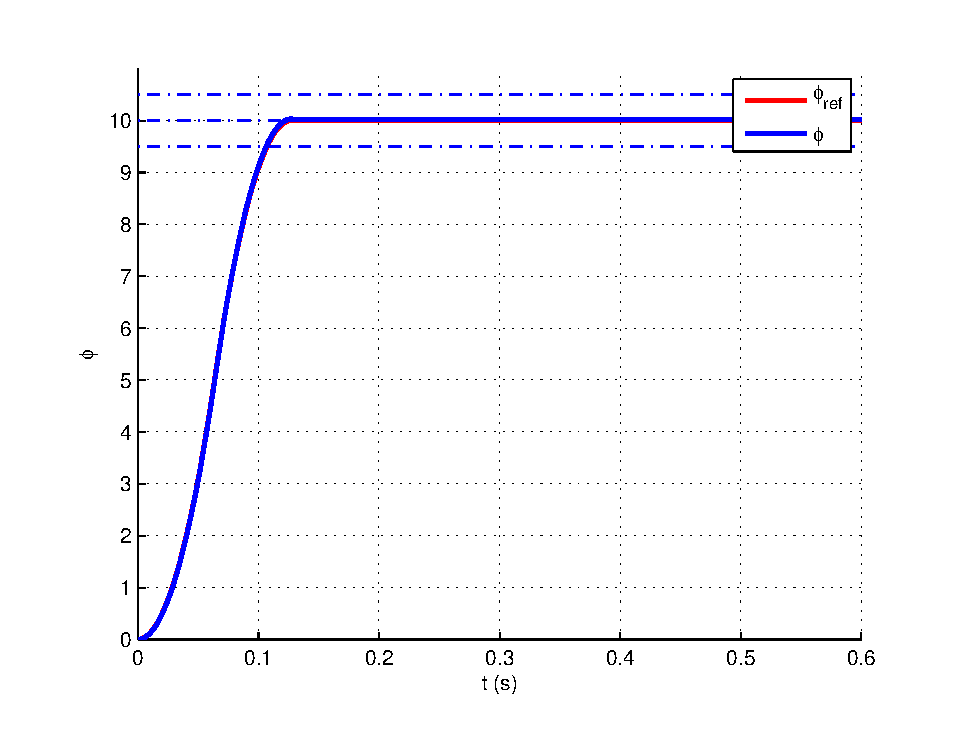
\includegraphics[width=\columnwidth]{fig/resultModelControl10.eps}
   \caption{$Rs = 10$[rad]}
  \end{subfigure}
  \begin{subfigure}[b]{\linewidth}
  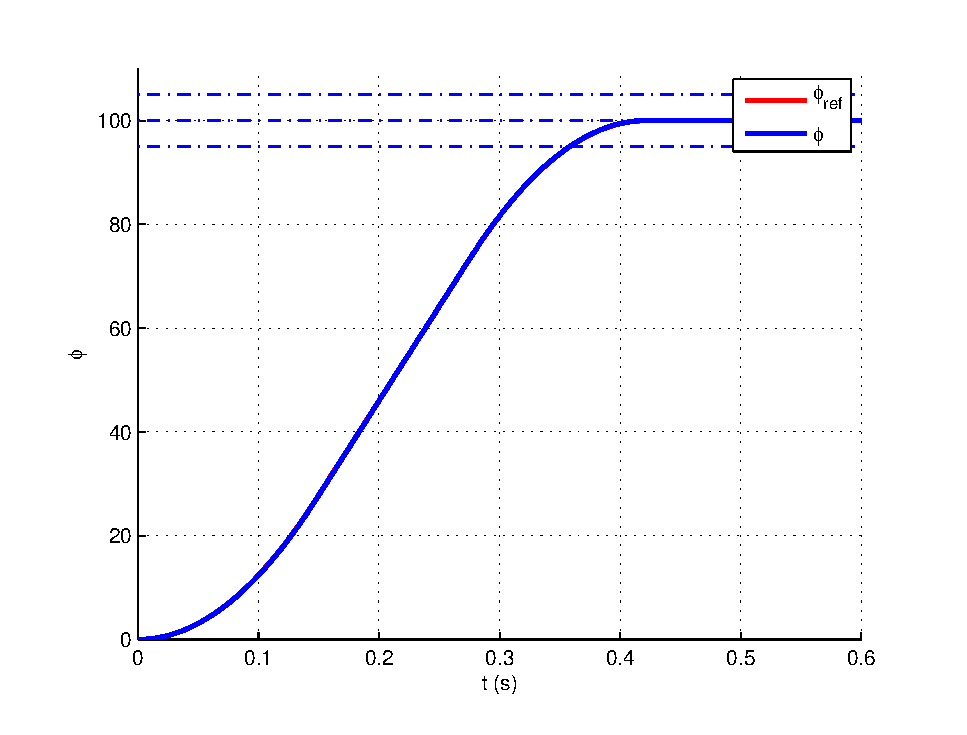
\includegraphics[width=\columnwidth]{fig/resultModelControl100.eps}
   \caption{$Rs = 100$[rad]}
  \end{subfigure}

 \caption{Position controller}
 \label{resultModelfollowing}
\end{figure}



